
%% bare_jrnl.tex
%% V1.3
%% 2007/01/11
%% by Michael Shell
%% see http://www.michaelshell.org/
%% for current contact information.
%%
%% This is a skeleton file demonstrating the use of IEEEtran.cls
%% (requires IEEEtran.cls version 1.7 or later) with an IEEE journal paper.
%%
%% Support sites:
%% http://www.michaelshell.org/tex/ieeetran/
%% http://www.ctan.org/tex-archive/macros/latex/contrib/IEEEtran/
%% and
%% http://www.ieee.org/



% *** Authors should verify (and, if needed, correct) their LaTeX system  ***
% *** with the testflow diagnostic prior to trusting their LaTeX platform ***
% *** with production work. IEEE's font choices can trigger bugs that do  ***
% *** not appear when using other class files.                            ***
% The testflow support page is at:
% http://www.michaelshell.org/tex/testflow/


%%*************************************************************************
%% Legal Notice:
%% This code is offered as-is without any warranty either expressed or
%% implied; without even the implied warranty of MERCHANTABILITY or
%% FITNESS FOR A PARTICULAR PURPOSE! 
%% User assumes all risk.
%% In no event shall IEEE or any contributor to this code be liable for
%% any damages or losses, including, but not limited to, incidental,
%% consequential, or any other damages, resulting from the use or misuse
%% of any information contained here.
%%
%% All comments are the opinions of their respective authors and are not
%% necessarily endorsed by the IEEE.
%%
%% This work is distributed under the LaTeX Project Public License (LPPL)
%% ( http://www.latex-project.org/ ) version 1.3, and may be freely used,
%% distributed and modified. A copy of the LPPL, version 1.3, is included
%% in the base LaTeX documentation of all distributions of LaTeX released
%% 2003/12/01 or later.
%% Retain all contribution notices and credits.
%% ** Modified files should be clearly indicated as such, including  **
%% ** renaming them and changing author support contact information. **
%%
%% File list of work: IEEEtran.cls, IEEEtran_HOWTO.pdf, bare_adv.tex,
%%                    bare_conf.tex, bare_jrnl.tex, bare_jrnl_compsoc.tex
%%*************************************************************************

% Note that the a4paper option is mainly intended so that authors in
% countries using A4 can easily print to A4 and see how their papers will
% look in print - the typesetting of the document will not typically be
% affected with changes in paper size (but the bottom and side margins will).
% Use the testflow package mentioned above to verify correct handling of
% both paper sizes by the user's LaTeX system.
%
% Also note that the "draftcls" or "draftclsnofoot", not "draft", option
% should be used if it is desired that the figures are to be displayed in
% draft mode.
%
\documentclass[10pt, journal, letterpaper, onecolumn, draftcls]{IEEEtran}
\usepackage{blindtext}
\usepackage{graphicx}
\usepackage{subfigure}
% Some very useful LaTeX packages include:
% (uncomment the ones you want to load)


% *** MISC UTILITY PACKAGES ***
%
%\usepackage{ifpdf}
% Heiko Oberdiek's ifpdf.sty is very useful if you need conditional
% compilation based on whether the output is pdf or dvi.
% usage:
% \ifpdf
%   % pdf code
% \else
%   % dvi code
% \fi
% The latest version of ifpdf.sty can be obtained from:
% http://www.ctan.org/tex-archive/macros/latex/contrib/oberdiek/
% Also, note that IEEEtran.cls V1.7 and later provides a builtin
% \ifCLASSINFOpdf conditional that works the same way.
% When switching from latex to pdflatex and vice-versa, the compiler may
% have to be run twice to clear warning/error messages.


\usepackage{tikz}
\usetikzlibrary{arrows.meta,decorations,decorations.text,backgrounds,arrows,shapes,intersections,calc,hobby}




% *** CITATION PACKAGES ***
%
\usepackage{cite}
% cite.sty was written by Donald Arseneau
% V1.6 and later of IEEEtran pre-defines the format of the cite.sty package
% \cite{} output to follow that of IEEE. Loading the cite package will
% result in citation numbers being automatically sorted and properly
% "compressed/ranged". e.g., [1], [9], [2], [7], [5], [6] without using
% cite.sty will become [1], [2], [5]--[7], [9] using cite.sty. cite.sty's
% \cite will automatically add leading space, if needed. Use cite.sty's
% noadjust option (cite.sty V3.8 and later) if you want to turn this off.
% cite.sty is already installed on most LaTeX systems. Be sure and use
% version 4.0 (2003-05-27) and later if using hyperref.sty. cite.sty does
% not currently provide for hyperlinked citations.
% The latest version can be obtained at:
% http://www.ctan.org/tex-archive/macros/latex/contrib/cite/
% The documentation is contained in the cite.sty file itself.






% *** GRAPHICS RELATED PACKAGES ***
%
\ifCLASSINFOpdf
  % \usepackage[pdftex]{graphicx}
  % declare the path(s) where your graphic files are
  % \graphicspath{{../pdf/}{../jpeg/}}
  % and their extensions so you won't have to specify these with
  % every instance of \includegraphics
  % \DeclareGraphicsExtensions{.pdf,.jpeg,.png}
\else
  % or other class option (dvipsone, dvipdf, if not using dvips). graphicx
  % will default to the driver specified in the system graphics.cfg if no
  % driver is specified.
  % \usepackage[dvips]{graphicx}
  % declare the path(s) where your graphic files are
  % \graphicspath{{../eps/}}
  % and their extensions so you won't have to specify these with
  % every instance of \includegraphics
  % \DeclareGraphicsExtensions{.eps}
\fi
% graphicx was written by David Carlisle and Sebastian Rahtz. It is
% required if you want graphics, photos, etc. graphicx.sty is already
% installed on most LaTeX systems. The latest version and documentation can
% be obtained at: 
% http://www.ctan.org/tex-archive/macros/latex/required/graphics/
% Another good source of documentation is "Using Imported Graphics in
% LaTeX2e" by Keith Reckdahl which can be found as epslatex.ps or
% epslatex.pdf at: http://www.ctan.org/tex-archive/info/
%
% latex, and pdflatex in dvi mode, support graphics in encapsulated
% postscript (.eps) format. pdflatex in pdf mode supports graphics
% in .pdf, .jpeg, .png and .mps (metapost) formats. Users should ensure
% that all non-photo figures use a vector format (.eps, .pdf, .mps) and
% not a bitmapped formats (.jpeg, .png). IEEE frowns on bitmapped formats
% which can result in "jaggedy"/blurry rendering of lines and letters as
% well as large increases in file sizes.
%
% You can find documentation about the pdfTeX application at:
% http://www.tug.org/applications/pdftex





% *** MATH PACKAGES ***
%
\usepackage[cmex10]{amsmath}
% A popular package from the American Mathematical Society that provides
% many useful and powerful commands for dealing with mathematics. If using
% it, be sure to load this package with the cmex10 option to ensure that
% only type 1 fonts will utilized at all point sizes. Without this option,
% it is possible that some math symbols, particularly those within
% footnotes, will be rendered in bitmap form which will result in a
% document that can not be IEEE Xplore compliant!
%
% Also, note that the amsmath package sets \interdisplaylinepenalty to 10000
% thus preventing page breaks from occurring within multiline equations. Use:
%\interdisplaylinepenalty=2500
% after loading amsmath to restore such page breaks as IEEEtran.cls normally
% does. amsmath.sty is already installed on most LaTeX systems. The latest
% version and documentation can be obtained at:
% http://www.ctan.org/tex-archive/macros/latex/required/amslatex/math/





% *** SPECIALIZED LIST PACKAGES ***
%
%\usepackage{algorithmic}
% algorithmic.sty was written by Peter Williams and Rogerio Brito.
% This package provides an algorithmic environment fo describing algorithms.
% You can use the algorithmic environment in-text or within a figure
% environment to provide for a floating algorithm. Do NOT use the algorithm
% floating environment provided by algorithm.sty (by the same authors) or
% algorithm2e.sty (by Christophe Fiorio) as IEEE does not use dedicated
% algorithm float types and packages that provide these will not provide
% correct IEEE style captions. The latest version and documentation of
% algorithmic.sty can be obtained at:
% http://www.ctan.org/tex-archive/macros/latex/contrib/algorithms/
% There is also a support site at:
% http://algorithms.berlios.de/index.html
% Also of interest may be the (relatively newer and more customizable)
% algorithmicx.sty package by Szasz Janos:
% http://www.ctan.org/tex-archive/macros/latex/contrib/algorithmicx/




% *** ALIGNMENT PACKAGES ***
%
%\usepackage{array}
% Frank Mittelbach's and David Carlisle's array.sty patches and improves
% the standard LaTeX2e array and tabular environments to provide better
% appearance and additional user controls. As the default LaTeX2e table
% generation code is lacking to the point of almost being broken with
% respect to the quality of the end results, all users are strongly
% advised to use an enhanced (at the very least that provided by array.sty)
% set of table tools. array.sty is already installed on most systems. The
% latest version and documentation can be obtained at:
% http://www.ctan.org/tex-archive/macros/latex/required/tools/


%\usepackage{mdwmath}
%\usepackage{mdwtab}
% Also highly recommended is Mark Wooding's extremely powerful MDW tools,
% especially mdwmath.sty and mdwtab.sty which are used to format equations
% and tables, respectively. The MDWtools set is already installed on most
% LaTeX systems. The lastest version and documentation is available at:
% http://www.ctan.org/tex-archive/macros/latex/contrib/mdwtools/


% IEEEtran contains the IEEEeqnarray family of commands that can be used to
% generate multiline equations as well as matrices, tables, etc., of high
% quality.


%\usepackage{eqparbox}
% Also of notable interest is Scott Pakin's eqparbox package for creating
% (automatically sized) equal width boxes - aka "natural width parboxes".
% Available at:
% http://www.ctan.org/tex-archive/macros/latex/contrib/eqparbox/





% *** SUBFIGURE PACKAGES ***
%\usepackage[tight,footnotesize]{subfigure}
% subfigure.sty was written by Steven Douglas Cochran. This package makes it
% easy to put subfigures in your figures. e.g., "Figure 1a and 1b". For IEEE
% work, it is a good idea to load it with the tight package option to reduce
% the amount of white space around the subfigures. subfigure.sty is already
% installed on most LaTeX systems. The latest version and documentation can
% be obtained at:
% http://www.ctan.org/tex-archive/obsolete/macros/latex/contrib/subfigure/
% subfigure.sty has been superceeded by subfig.sty.



%\usepackage[caption=false]{caption}
%\usepackage[font=footnotesize]{subfig}
% subfig.sty, also written by Steven Douglas Cochran, is the modern
% replacement for subfigure.sty. However, subfig.sty requires and
% automatically loads Axel Sommerfeldt's caption.sty which will override
% IEEEtran.cls handling of captions and this will result in nonIEEE style
% figure/table captions. To prevent this problem, be sure and preload
% caption.sty with its "caption=false" package option. This is will preserve
% IEEEtran.cls handing of captions. Version 1.3 (2005/06/28) and later 
% (recommended due to many improvements over 1.2) of subfig.sty supports
% the caption=false option directly:
%\usepackage[caption=false,font=footnotesize]{subfig}
%
% The latest version and documentation can be obtained at:
% http://www.ctan.org/tex-archive/macros/latex/contrib/subfig/
% The latest version and documentation of caption.sty can be obtained at:
% http://www.ctan.org/tex-archive/macros/latex/contrib/caption/




% *** FLOAT PACKAGES ***
%
%\usepackage{fixltx2e}
% fixltx2e, the successor to the earlier fix2col.sty, was written by
% Frank Mittelbach and David Carlisle. This package corrects a few problems
% in the LaTeX2e kernel, the most notable of which is that in current
% LaTeX2e releases, the ordering of single and double column floats is not
% guaranteed to be preserved. Thus, an unpatched LaTeX2e can allow a
% single column figure to be placed prior to an earlier double column
% figure. The latest version and documentation can be found at:
% http://www.ctan.org/tex-archive/macros/latex/base/



%\usepackage{stfloats}
% stfloats.sty was written by Sigitas Tolusis. This package gives LaTeX2e
% the ability to do double column floats at the bottom of the page as well
% as the top. (e.g., "\begin{figure*}[!b]" is not normally possible in
% LaTeX2e). It also provides a command:
%\fnbelowfloat
% to enable the placement of footnotes below bottom floats (the standard
% LaTeX2e kernel puts them above bottom floats). This is an invasive package
% which rewrites many portions of the LaTeX2e float routines. It may not work
% with other packages that modify the LaTeX2e float routines. The latest
% version and documentation can be obtained at:
% http://www.ctan.org/tex-archive/macros/latex/contrib/sttools/
% Documentation is contained in the stfloats.sty comments as well as in the
% presfull.pdf file. Do not use the stfloats baselinefloat ability as IEEE
% does not allow \baselineskip to stretch. Authors submitting work to the
% IEEE should note that IEEE rarely uses double column equations and
% that authors should try to avoid such use. Do not be tempted to use the
% cuted.sty or midfloat.sty packages (also by Sigitas Tolusis) as IEEE does
% not format its papers in such ways.


%\ifCLASSOPTIONcaptionsoff
%  \usepackage[nomarkers]{endfloat}
% \let\MYoriglatexcaption\caption
% \renewcommand{\caption}[2][\relax]{\MYoriglatexcaption[#2]{#2}}
%\fi
% endfloat.sty was written by James Darrell McCauley and Jeff Goldberg.
% This package may be useful when used in conjunction with IEEEtran.cls'
% captionsoff option. Some IEEE journals/societies require that submissions
% have lists of figures/tables at the end of the paper and that
% figures/tables without any captions are placed on a page by themselves at
% the end of the document. If needed, the draftcls IEEEtran class option or
% \CLASSINPUTbaselinestretch interface can be used to increase the line
% spacing as well. Be sure and use the nomarkers option of endfloat to
% prevent endfloat from "marking" where the figures would have been placed
% in the text. The two hack lines of code above are a slight modification of
% that suggested by in the endfloat docs (section 8.3.1) to ensure that
% the full captions always appear in the list of figures/tables - even if
% the user used the short optional argument of \caption[]{}.
% IEEE papers do not typically make use of \caption[]'s optional argument,
% so this should not be an issue. A similar trick can be used to disable
% captions of packages such as subfig.sty that lack options to turn off
% the subcaptions:
% For subfig.sty:
% \let\MYorigsubfloat\subfloat
% \renewcommand{\subfloat}[2][\relax]{\MYorigsubfloat[]{#2}}
% For subfigure.sty:
% \let\MYorigsubfigure\subfigure
% \renewcommand{\subfigure}[2][\relax]{\MYorigsubfigure[]{#2}}
% However, the above trick will not work if both optional arguments of
% the \subfloat/subfig command are used. Furthermore, there needs to be a
% description of each subfigure *somewhere* and endfloat does not add
% subfigure captions to its list of figures. Thus, the best approach is to
% avoid the use of subfigure captions (many IEEE journals avoid them anyway)
% and instead reference/explain all the subfigures within the main caption.
% The latest version of endfloat.sty and its documentation can obtained at:
% http://www.ctan.org/tex-archive/macros/latex/contrib/endfloat/
%
% The IEEEtran \ifCLASSOPTIONcaptionsoff conditional can also be used
% later in the document, say, to conditionally put the References on a 
% page by themselves.





% *** PDF, URL AND HYPERLINK PACKAGES ***
%
%\usepackage{url}
% url.sty was written by Donald Arseneau. It provides better support for
% handling and breaking URLs. url.sty is already installed on most LaTeX
% systems. The latest version can be obtained at:
% http://www.ctan.org/tex-archive/macros/latex/contrib/misc/
% Read the url.sty source comments for usage information. Basically,
% \url{my_url_here}.


%\usepackage{amsmath}
\usepackage{amssymb}
%\usepackage{mathtools}

%\usepackage{algorithm}
%\usepackage{algpseudocode}
%\usepackage{pifont}

\usepackage{multirow}
\usepackage{hhline}
\usepackage{longtable}
\usepackage{tabu}

\usepackage{hyperref}
\usepackage{cleveref}

% *** Do not adjust lengths that control margins, column widths, etc. ***
% *** Do not use packages that alter fonts (such as pslatex).         ***
% There should be no need to do such things with IEEEtran.cls V1.6 and later.
% (Unless specifically asked to do so by the journal or conference you plan
% to submit to, of course. )


% correct bad hyphenation here
\hyphenation{op-tical net-works semi-conduc-tor}

\DeclareMathOperator*{\argmin}{arg\,min}

\begin{document}
%
% paper title
% can use linebreaks \\ within to get better formatting as desired
\title{Automatic Parameter Estimation for Graph-Cut Chan-Vese for Fluorescence Image Binarization}
%
%
% author names and IEEE memberships
% note positions of commas and nonbreaking spaces ( ~ ) LaTeX will not break
% a structure at a ~ so this keeps an author's name from being broken across
% two lines.
% use \thanks{} to gain access to the first footnote area
% a separate \thanks must be used for each paragraph as LaTeX2e's \thanks
% was not built to handle multiple paragraphs
%

\author{Ryan~Naidoo, Jules-Raymond~Tapamo}

% note the % following the last \IEEEmembership and also \thanks - 
% these prevent an unwanted space from occurring between the last author name
% and the end of the author line. i.e., if you had this:
% 
% \author{....lastname \thanks{...} \thanks{...} }
%                     ^------------^------------^----Do not want these spaces!
%
% a space would be appended to the last name and could cause every name on that
% line to be shifted left slightly. This is one of those "LaTeX things". For
% instance, "\textbf{A} \textbf{B}" will typeset as "A B" not "AB". To get
% "AB" then you have to do: "\textbf{A}\textbf{B}"
% \thanks is no different in this regard, so shield the last } of each \thanks
% that ends a line with a % and do not let a space in before the next \thanks.
% Spaces after \IEEEmembership other than the last one are OK (and needed) as
% you are supposed to have spaces between the names. For what it is worth,
% this is a minor point as most people would not even notice if the said evil
% space somehow managed to creep in.



% The paper headers
\markboth{Journal of \LaTeX\ Class Files,~Vol.~6, No.~1, January~2017}%
{Shell \MakeLowercase{\textit{et al.}}: Bare Demo of IEEEtran.cls for Journals}
% The only time the second header will appear is for the odd numbered pages
% after the title page when using the twoside option.
% 
% *** Note that you probably will NOT want to include the author's ***
% *** name in the headers of peer review papers.                   ***
% You can use \ifCLASSOPTIONpeerreview for conditional compilation here if
% you desire.




% If you want to put a publisher's ID mark on the page you can do it like
% this:
%\IEEEpubid{0000--0000/00\$00.00~\copyright~2007 IEEE}
% Remember, if you use this you must call \IEEEpubidadjcol in the second
% column for its text to clear the IEEEpubid mark.



% use for special paper notices
%\IEEEspecialpapernotice{(Invited Paper)}




% make the title area
\maketitle


\begin{abstract}
The detailed analytical studies of microscopic organisms and such have played a vital role in a host of fields ranging from the simple curiosity of what goes on at the mirco-level to studying the behaviour of cancerous cells. Fluorescence images are generated by the thousands to study these phenomena. The rate at which we're able to gather data outweighs the rate at which we're able to accurately study it.
%The key to efficient and effective study lies heavily on the ability to bring into focus what is needful and discard everything else. In the study of fluorescence images, it is absolutely critical that the object be segmented accuratetly and quickly.
%The optical challenges present in fluorescence images make it a very unique class of image data, as such, other segmentation parameters settings cannot be readily applied to it. One must start at the ground level to find the optimal parameters for accurate segmentation; which is tedious and an ineffective use of time. There is also a large variance in the types of images within the set of fluorescence images and hard-coded parameters are quick to hit a brick wall, and once again it is back to the drawing board for searching out the correct parameters for segmentation.
The purpose of this study is too investigate the properties of fluorescence images and leverage that understanding to develop a technique that is able to automatically produce image-specific accurate parameter settings for segmentation of the object of interest.
In this paper, we present a novel parameter estimation technique for the graph cut implementation of the Chan-Vese approximation of the Mumford-Shah functional for image segmentation.
The effectiveness of the technique is demonstrated through a set of experiments with real images.
%These images are chosen such that the set has broad coverage wit the type of images that are commonly obtained in fluorescence imaging.
We pit our approach against two other common paramter settings. Our segmentation scheme is highly robust and produces superior segmentation results with an average accuracy of 93.533\%.
\end{abstract}
% IEEEtran.cls defaults to using nonbold math in the Abstract.
% This preserves the distinction between vectors and scalars. However,
% if the journal you are submitting to favors bold math in the abstract,
% then you can use LaTeX's standard command \boldmath at the very start
% of the abstract to achieve this. Many IEEE journals frown on math
% in the abstract anyway.

% Note that keywords are not normally used for peerreview papers.
\begin{IEEEkeywords}
Image segmentation, graph cuts, fluorescence, active-contours, Chan-Vese, Mumford-Shah.
\end{IEEEkeywords}






% For peer review papers, you can put extra information on the cover
% page as needed:
% \ifCLASSOPTIONpeerreview
% \begin{center} \bfseries EDICS Category: 3-BBND \end{center}
% \fi
%
% For peerreview papers, this IEEEtran command inserts a page break and
% creates the second title. It will be ignored for other modes.
%\IEEEpeerreviewmaketitle



\section{Introduction}
\label{sec:Intro}
\textbf{Lay the foundation to present the problem.} Amount of images. Problems with the images. The type of solutions available that miss solving the problem.
\textbf{Present the problem.}
\textbf{What solution do we seek.}
\textbf{Scope of the paper.}
\textbf{Other tried approaches. What are their weaknesses? What did they sacrifice to get that scheme or result.}
\textbf{What schemes will we be competing with.}
\textbf{Organisation.} Firstly, we begin in \Cref{sec:CVformulation} with a brief introduction to the Chan-Vese formulation of the  Mumford-Shah energy functional. Then in \Cref{sec:CVgraphcut} we introduce the graph-cut approach to image segmentation and how it is used to solve the Chan-Vese image segmentation problem. We then develop the proposed technique for parameter estimation in \Cref{sec:Proptechnique}. In \Cref{sec:Expresults} we show some experimental results and demonstrate the efficiency and robustness of this scheme. We also compare the proposed scheme against two other well-known schemes. Our concluding remarks are shown in \Cref{sec:Conc}.

\section{Chan-Vese Formulation of the Mumford-Shah Energy Functional}
\label{sec:CVformulation}
The Mumford-Shah evolution energy functional is a segmentation model to be minimised over an approximation image $u$ of the input image $u_0$. The level set representation of the Mumford-Shah energy function is 
\begin{equation}
\begin{split}
	F(c_1, c_2, \phi) & = \mu \int_\Omega \delta(\phi(x,y))|\nabla\phi(x,y)|dxdy \\
	& + \nu \int_\Omega H(\phi(x,y))dxdy \\
	& + \lambda_1 \int_\Omega |u(x,y)-c_1|^2H(\phi(x,y))dxdy \\
	& + \lambda_2 \int_\Omega |u(x,y)-c_2|^2(1-H(\phi(x,y)))dxdy,
	\end{split}
	\label{eq:mumfordshahfunction}
\end{equation}

where $\lambda_1, \, \lambda_2, \, \mu, \text{ and } \nu$ are fixed parameters such that $\lambda_1, \lambda_2 > 0$ and $\mu, \nu \geq 0$.  $u(x,y)$ is the image, $H(\cdot)$ is the Heaviside step function, $\delta(\cdot)$ is the Dirac delta function, $\Phi$ is an open unbounded subset of $\Re^2$ and $\phi:\Omega \rightarrow \mathbb{R}$ is the level set function, such that:
\begin{equation}
	\begin{split}
	\omega & = \{(x,y) \in \Omega|\Phi(x_p)>0\} \\
	\bar{\omega} & = \{(x,y) \in \Omega|\Phi(x_p)<0\} \\
	C = \partial\omega & = \{(x,y) \in \Omega|\Phi(x_p)=0\},
	\end{split}
	\label{eq:levelsetrepresentation}
\end{equation}

$c_1$ and $c_2$ are the arithmetic means of the intensities in the regions of $u$ defined by the masks $H(\phi(x,y)$ and $1-H(\phi(x,y)$ respectively. The piece-wise smooth approximation of the image is then 
\begin{equation}
	u(x,y) = c_1 H(\phi(x,y)) + c_2(1-H(\phi(x,y))).
	\label{eq:piecewiseapproximation}
\end{equation}

\subsection{Discretising the Mumford-Shah Functional}
With the exception of the second term in \Cref{eq:mumfordshahfunction}, the remaining terms can be represented discretely very easily. For each pixel $p \in \Omega$, let $x_p$ be a binary variable such that
\begin{equation}
	x_p = 
	\begin{cases} 
	0 & \phi(p)\leq 0 \\
	1 & \phi(p)> 0
	\end{cases}
\end{equation}

The means can now be calculated using 
\begin{equation}
	c_1 = \frac{\sum_p u(x,y)x_p}{\sum_p x_p},
\end{equation}
\begin{equation}
	c_2 = \frac{\sum_p u(x,y)(1-x_p)}{\sum_p (1-x_p)}.
\end{equation}

For simplification, set $\nu = 0$. Kolmogorov and Boykov in [] used the Cauchy-Crofton thereom to approximate the length of a contour $C$ by counting the number of intersections with the line $L$. By using this approximation, it can be shown that the Euclidean contour length can
 be expressed as
\begin{equation}
	\lVert C \rVert_E = \sum_{p,q \in e_k} w_k( x_p(1-x_q) + x_q(1-x_p)).
\end{equation}

The fully discrete form of \Cref{eq:mumfordshahfunction} is
\begin{equation}
	\begin{split}
	F(x_1, \ldots, x_n) & = \mu \sum_{p,q \in e_k} w_k( x_p(1-x_q) + x_q(1-x_p)) \\
	& + \lambda_1 \sum_p |u(x,y)-c_1|^2x_p \\
	& + \lambda_2 \sum_p |u(x,y)-c_2|^2(1-x_p)
	\end{split}
	\label{eq:discretemumfordshah}
\end{equation}

\section{Graph-Cut Model for Chan-Vese Segmentation}
\label{sec:CVgraphcut}
Graph Cuts are a well known optimisation problem in Combinatronics. Due to the duality known as the Max-Flow Min-Cut Thereom, there are several fast algorithms to find the mincut. Typically, it's easier to solve the the Max-Flow problem and bulk of the optimised algorithms are designed on Max-flow algorithms. Graph Cuts were unsuccesfully introduce into Computer Vision by Greig \textit{et al.} [] and was later popularised by Kolmogorov [].

A graph $G=(V, E)$ is a set of vertices/nodes $V$, and a set of directed edges $E$ with positive weights/capacities that connect these vertices. We let $uv$ be a directed edge going from $u$ to $v$. The weight of the edge is denoted by $c(u, v)$. In the 2-label graph cut, there are two more vertices that don't correspond to any pixels. These are the source $s$ and the sink $t$. All other nodes are directly connected to both the source and the sink. Therefore, a cut on $G$ is a partioning of $V$ into two disjoint connected sets $(V_s, V_t)$ such that $s \in V_s$ and $t \in V_t$. The cost of the cut is calculated as

\begin{equation}
	c(V_s, V_t) = \sum_{i \in V_s, j \in V_t}c(i, j).
\end{equation}

Graph cuts are used to minimise energies of the form
\begin{equation}
	\argmin_{x \in \{0,1\}^m}	E(x) = \sum_i E^i(x_i) + \sum_{i<j}E^{i,j}(x_i, x_j).
	\label{eq:graphcutenergyform}
\end{equation}

For an energy to be graph-representable, the pairwise interaction potentials must be submodular [], i.e. it must adhere to the following constraint.
\begin{equation}
	E^{i,j}(0,0) + E^{i,j}(1,1) \leq E^{i,j}(0,1) + E^{i,j}(1,0), \, \forall i < j.
\end{equation}

It has been shown in [] that \Cref{eq:discretemumfordshah} is submodular and hence the optimal solution can be found via graph cuts. The data and regularisation energy respectively in \Cref{eq:graphcutenergyform} is
\begin{equation}
	E^i(x_i) = \lambda_1 |u(x,y)-c_1|^2 x_i + \lambda_2 |u(x,y)-c_2|^2 (1-x_i)
\end{equation}
\begin{equation}
	E^{i,j}(x_i,x_j) = (x_i + x_j - 2x_ix_j)w_{ij}
\end{equation}

\section{Chan-Vese Parameter Estimation for Graph-Cuts}
\label{sec:Proptechnique}
In this section we introduce the proposed method for Chan-Vese parameter estimation for graph-cuts. Previous parameter estimation schemes focussed on a certain genre of images or image characteristics, and these resulted in a set of hard-coded parameter settings. These hard-coded parameters are not very useful in producing consistent reults in the greater applications of image segmentation even within the fields for which they were optimised.

We devise a novel weighting scheme for the graph and propose a general parameter estimation technique in which the parameters adapt themselves to the image. We achieve this not by focusing on the parameters, but rather the relationship between the parameters. We then isolate these relationships in proxy relational parameters which we then tune for fluorescence images.

\subsection{Proposed Technique}
We first explain the method used to weight the graph. We begin by normalising the data and smoothing connections. We use the Euclidean distance to weighting of the edges connecting adjacent nodes, i.e. diagonally adjacent node in the 8-connected graph would be scaled by $\frac{1}{\sqrt{2}}$, etc.

The image pixel values are also normalised i.e. $p \in [0,1]$, where $p$ is the pixel value of the $i$-th pixel in the image. The edge connecting the source to the node which corresponds to pixel $i$ is given by  $E^i(0)|_{i=p} = \lambda_0|p-c_0|^2$. This is how far away the pixel is from the average foreground/object pixel intensity $c_0$.  Similarly, the weight of the connection from the node to the sink is given by $E^i(1)|_{i=p}=\lambda_1|p-c_1|^2$, i.e. how far away the pixel is from the average background pixel intensity $c_1$.

Whether a node is connected to the source or the sink after segmentation depends on its connections which are wighted by the previously defined energy functions. It behooves use to study then, the relationship between the energy functions. We see that there are two tunable parameters namely $\lambda_0$ and $\lambda_1$. It is the relationship between these two parameter that heavily influence the output. We simplify and explicitely formalise the relationship between and set
\begin{equation}
	\lambda_0 = \alpha\lambda_1.
	\label{eq:l0l1dependancy}
\end{equation}
Forcing this relationship make further analysis simpler and more intuitive. An immediate constraint is $\alpha > 0$, since we require all data conenctions to be positive, i.e $E^i(0), E^i(1) \geq 0$.

We will now analyse the flow through a single node in the 8-connected graph, we use \Cref{fig:singlenodeconstruction} to facilitate our explanation. Two nodes are maximally connected if their corresponding pixel values are the same, i.e. there is no difference between them. Let this value be $\mu$. Hence, the maximum possible flow into or out of a node to its neighbours is
\begin{equation}
	f_{max} = 4\mu + 4\frac{\mu}{\sqrt{2}} = \mu \left( 2\sqrt{2} + 4\right).
	\label{eq:neighbourhoodsaturation}
\end{equation}

We know that for a node $p$ to belong to the source set, i.e. $ p \in S$, the incoming flow from the source must completely saturate all outlets. This can be expressed as
\begin{equation}
	E^i(0) > E^i(1) + \mu \left( 2\sqrt{2} + 4\right).
	\label{eq:sourcesaturation}
\end{equation}
Similarly, to guarantee the node will be in the sink set, $p \in T$, we have
\begin{equation}
	E^i(1) > E^i(0) + \mu \left( 2\sqrt{2} + 4\right).
	\label{eq:sinksaturation}
\end{equation}

\tikzstyle{vertex}=[circle,thick,draw]
\begin{figure}[!h]
	\centering
	\begin{tikzpicture}[scale=1.0]
	\draw (0,0) -- (2,0);
	\draw (0,0) -- (-2,0);
	\draw (0,0) -- (0,1) node[right] {$\mu$} -- (0,2);
	\draw (0,0) -- (0,-2);
	
	\draw (0,0) -- (-2,2);
	\draw (0,0) -- (2,2);
	\draw (0,0) -- (-1,-1) node[right] {$\frac{\mu}{\sqrt{2}}$} -- (-2,-2);
	\draw (0,0) -- (2,-2);
	
	\draw[red,thick] (-5,2) .. controls(-4,-1) and (-2,1.5) .. (0,0);
	\draw[red,->,thick] (-2.5,0.48) -- (-2.4,0.485) node[above] {$E^i(0)$};
	\node[vertex,red,fill=red!20] at (-5,2) {$S$};
	\draw[blue,thick] (5,-2) .. controls(4,1) and (2,-1.5) .. (0,0);
	\draw[blue,<-,thick] (2.5,-0.48) -- (2.4,-0.485) node[below] {$E^i(1)$};
	\node[vertex,blue,fill=blue!20] at (5,-2) {$T$};
	
	\draw[fill=white] (0,0) circle (0.35);
	\draw[fill=black] (-2,0) circle (0.25);
	\draw[fill=black] (2,0) circle (0.25);
	
	\draw[fill=black] (0,2) circle (0.25);
	\draw[fill=black] (-2,2) circle (0.25);
	\draw[fill=black] (2,2) circle (0.25);
	
	\draw[fill=black] (0,-2) circle (0.25);
	\draw[fill=black] (-2,-2) circle (0.25);
	\draw[fill=black] (2,-2) circle (0.25);
	\end{tikzpicture}
	\caption{Fully connected single node.}
	\label{fig:singlenodeconstruction}
\end{figure}

To aid in understanding the energies, we use \Cref{fig:dataenergyplot}.

\begin{figure}[!t]
	\centering
	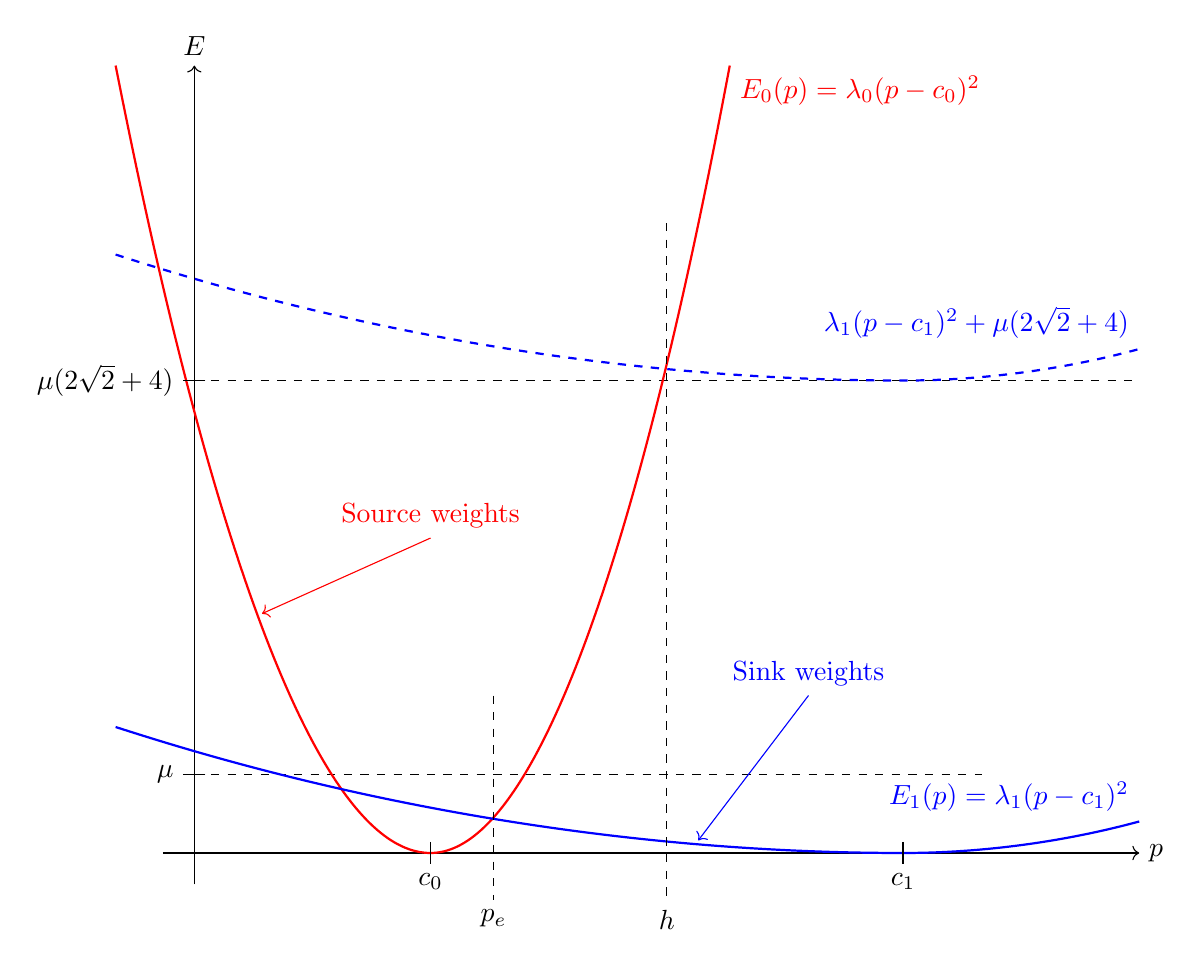
\begin{tikzpicture}[scale=2]
	\draw[->] (-0.2,0) -- (6,0) node[right] {$p$};
	\draw[->] (0,-0.2) -- (0,5) node[above] {$E$};
	
	\draw[dashed] (0,0.5) -- (5,0.5);
	\draw[dashed] (0,3) -- (6,3);
	\draw[red,thick] (-0.5,5) parabola bend (1.5,0) (3.4,5) node[below right] {$E_0(p) = \lambda_0 (p-c_0)^2$};
	\draw[blue,thick] (-0.5,0.8) parabola bend (4.5,0) (6,0.2) node[above left] {$E_1(p) = \lambda_1 (p-c_1)^2$};
	\draw[dashed,blue,thick] (-0.5,3.8) parabola bend (4.5,3) (6,3.2) node[above left] {$\lambda_1 (p-c_1)^2 + \mu(2\sqrt{2}+4)$};
	\draw[shift={(1.5,0)}] (0pt,2pt) -- (0pt,-2pt) node[below] {$c_0$};
	\draw[shift={(4.5,0)}] (0pt,2pt) -- (0pt,-2pt) node[below] {$c_1$};
	\draw[shift={(0,0.5)}] (2pt,0pt) -- (-2pt,0pt) node[left] {$\mu$};
	\draw[shift={(0,3)}] (2pt,0pt) -- (-2pt,0pt) node[left] {$\mu(2\sqrt{2}+4)$};
	
	\draw[dashed,black] (3.0,4) -- (3.0,-0.3) node[below] {$h$};
	\draw[dashed,black] (1.9,1) -- (1.9,-0.3) node[below] {$p_e$};
	%\draw[dashed,black] (0.94,1) -- (0.94,-0.3) node[below] {$p_e$};
	
	\draw[red,<-] (0.43,1.52) -- (1.5,2) node[above] {Source weights};
	\draw[blue,<-] (3.2,0.08) -- (3.9,1) node[above] {Sink weights};
	\end{tikzpicture}
	\caption{Data energy functions plot.}
	\label{fig:dataenergyplot}
\end{figure}

For quadratic energies with $0 < c_0 < c_1 < 1$, there is a point, between $c_0$ and $c_1$, where the incoming flow from the source completely saturates the sink with no excess remaining. This point, where the energies are equal, we call $p_e$, i.e. $E_0(p_e) = E_1(p_e)$. Taking into account the relation in \Cref{eq:l0l1dependancy}, this point of zero net flow is found to be
\begin{equation}
	p_e = c_0 + \frac{c_1-c_0}{\sqrt{\alpha} + 1}
	\label{eq:pe}
\end{equation}
The point where the energies are equal, $p_e$, is shown in \Cref{fig:dataenergyplot}.

We now shift our focus on the relationship between $p_e$ and $\alpha$. We see that $\alpha$ is the only tuneable parameter. From this inverse relationship we note three major points. These are
\begin{equation*}\begin{split}
	\text{if } \alpha=1, p_e=c_0+\frac{c_1-c_0}{1+\sqrt{1}} = \frac{c_0+c_1}{2} \hspace{30pt}&\text{(midpoint between $c_0$ and $c_1$)}\\
	\lim_{\alpha\to\infty}p_e = c_0\hspace{30pt} &\text{(maximum $\alpha$ yields lower-bound on $p_e$)}\\
	\lim_{\alpha\to0}p_e = c_1\hspace{30pt} &\text{(minimum $\alpha$ yields upper-bound on $p_e$)}
\end{split}\end{equation*}
This is relationship is shown graphically in \Cref{fig:alphaperelationship}.
\begin{figure}[!h]
	\centering
	\begin{tikzpicture}[scale=1]
	\draw[->] (0,0) -- (15,0) node[right] {$p$};
	\draw[shift={(3,0)}] (0pt,4pt) -- (0pt,-4pt) node[below] {$c_0$};
	\draw[shift={(12,0)}] (0pt,4pt) -- (0pt,-4pt) node[below] {$c_1$};
	\draw[dashed,black] (7.5,1.5) node[above] {$p_e = \frac{c_0+c_1}{2}$} -- (7.5,-0.3) node[below] {$\alpha=1$};
	\draw[black,->,thick] (7.5,0.5) -- (5.5,0.5) node[above] {increasing $\alpha$} -- (4.5,0.5);
	\draw[black,->,thick] (7.5,0.5) -- (9.5,0.5) node[above] {decreasing $\alpha$} -- (10.5,0.5);
	\end{tikzpicture}
	\caption{Relationship between $\alpha$ and $p_e$.}
	\label{fig:alphaperelationship}
\end{figure}

If we can make a good estimation for $p_e$, $c_0$ and $c_1$ for the segmentated image, then it can be shown that the corresponding $\alpha$ can be calculated as
\begin{equation}
	\alpha = \left( \frac{c_1-c_0}{p_e-c_0}-1 \right)^2
	\label{eq:alphaapproximation}
\end{equation}

When we calculated the intersection between the energies $p_e$, we ignored the other point that was out of the range $[c_0, c_1]$.Let this point be $p_{e^*}$. If this point is positive and $0<p_{e^*}<c_0$ then we must ensure that at no point within this range must the source flow saturate all outgoing edges. This forces a limit on how low $\mu$ can be. This is only of significant concern when $\alpha>1$. We only need to concern ourselves with the point $p=0$ as this is the point where the difference $E^i(0)-E^i(1)$ is the largest. Taking into account the relation in \Cref{eq:l0l1dependancy}, the lower-bound on $\mu$ can be shown to be 
\begin{equation}
	\mu > \frac{\lambda_1(\alpha c_0^2-c_1^2)}{C}
	\label{eq:mulowerbound}
\end{equation}
%\begin{equation}
%\mu > \frac{\lambda_1(\alpha c_0^2-c_1^2)}{\left( 2\sqrt{2} + 4\right)}
%\label{eq:mulowerbound}
%\end{equation}
We set $C=\left( 2\sqrt{2} + 4\right)$ which is the sum of all the attenuating factors of the edges connected to a node.

From \Cref{eq:sourcesaturation} we can see that there is a point beyond which all nodes which correspond to pixel value higher than that point will be saturated and have excess flow; this means that they will be in the source set. We will call this point the \textit{saturation point} and denote it by $h$. This is shown in \Cref{fig:dataenergyplot}. This point can be determined using
\begin{equation}
	h = \frac{(\alpha c_0-c_1)+\sqrt{\alpha(c_0-c_1)^2+\frac{C\mu}{\lambda_1}(\alpha-1)}}{\alpha-1}
	\label{eq:h}
\end{equation}
%\begin{equation}
%h = \frac{(\alpha c_0-c_1)+\sqrt{\alpha(c_0-c_1)^2+\frac{\mu(2\sqrt{2}+4)}{\lambda_1}(\alpha-1)}}{\alpha-1}
%\label{eq:h}
%\end{equation}
This point is marked off in \Cref{fig:dataenergyplot}.

Therefore, given good approximations for $c_0$, $c_1$, $\alpha$, $h$ and $\mu$, we can calculate the appropriate value for $\lambda_1$. This can be shown to be
\begin{equation}
	\lambda_1 = \frac{C\mu}{\alpha(h-c_0)^2-(h-c_1)^2}
	\label{eq:lambda1approximation}
\end{equation}
%\begin{equation}
%\lambda_1 = \frac{\mu(2\sqrt{2}+4)}{\alpha(h-c_0)^2-(h-c_1)^2}
%\label{eq:lambda1approximation}
%\end{equation}

The parameter estimation is based on the assumption that sufficiently good approximations for $c_0$, $c_1$, $p_e$ and $h$ can be obtained. By sufficiently good we are referring to the closeness to the values these parameters would be for an ideal segmentation. From these approximations, we calculate $\alpha$ using \Cref{eq:alphaapproximation}. The parameters $\mu$ and $\lambda_1$ are not separable, therefore we choose to set $\mu$. We can then calculate $\lambda_1$ using \Cref{eq:lambda1approximation}. Finally $\lambda_0$ can be calculated using \Cref{eq:l0l1dependancy}. In the next section we discuss how we make the guess for good approximations for the required parameters.

\subsection{Tuning the Proxy Parameters}
The properties of the images obtained in fluorescence microscopy imaging can be used to guide the parameter estimation process. We focus specifically on black background fluorescent images. Due to the fact that the predominant form of noise in the imaging system in Poisson distributed, we can further assume that the darker the background, the less noise that is present therein. The Poisson process also tells us that brighter regions exhibit a greater intensity variation due to the sampling process. Therefore, the curve for $E^i(1)$ is less convex than $E^i(0)$ as in \Cref{fig:dataenergyplot} and, resultantly, the value for $p_e$, in \Cref{fig:alphaperelationship}, is shifted to the left. This places a new lower-bound on $\alpha$ for fluorescence images
\begin{equation}
	\alpha \geq 1.
	\label{eq:alphalowerboundFM}
\end{equation}

The tuning process we used is as follows:
We manually segmented the fluorescent images in \Cref{fig:tuningset}. The segmentation results that were closest to the groundtruth were chosen and the corresponding proxy parameters were calculated for each image. The final setting for the proxy parameter was taken as the average value for each proxy parameter from all images. 

\def \myWidth {0.146}
\begin{figure}[!t]
	\centering
	\subfigure[Image 1]
	{
		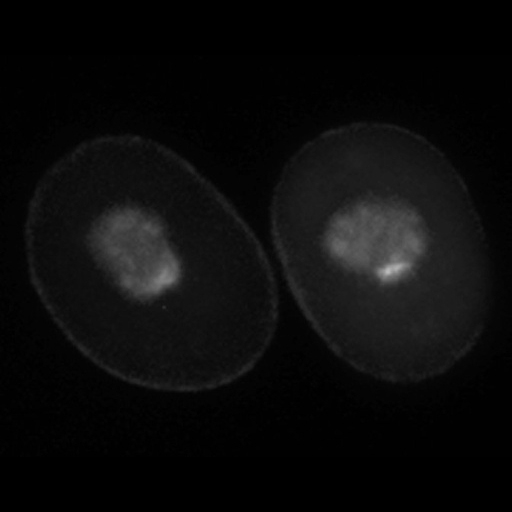
\includegraphics[width=\myWidth\columnwidth]{figures/cell_database_gray/1gray.jpg}
		\label{fig:1gray}
	}
	\subfigure[Image 2]
	{
		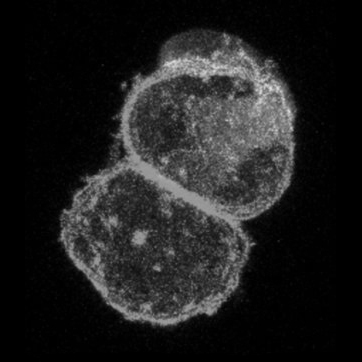
\includegraphics[width=\myWidth\columnwidth]{figures/cell_database_gray/2gray.jpg}
		\label{fig:2gray}
	}
	\subfigure[Image 3]
	{
		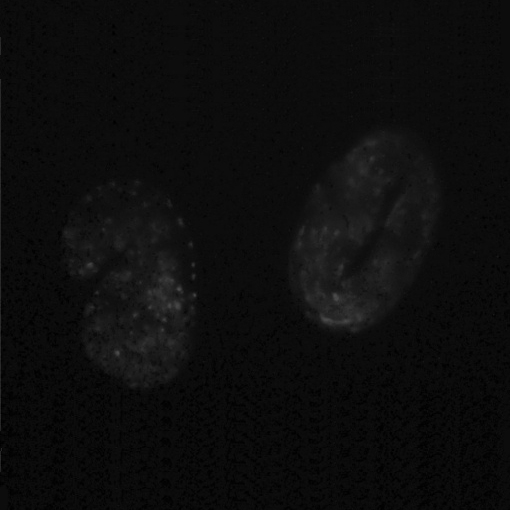
\includegraphics[width=\myWidth\columnwidth]{figures/cell_database_gray/3gray.jpg}
		\label{fig:3gray}
	}
	\subfigure[Image 4]
	{
		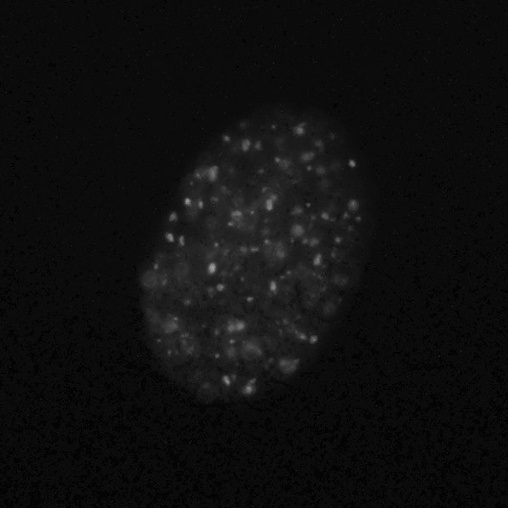
\includegraphics[width=\myWidth\columnwidth]{figures/cell_database_gray/4gray.jpg}
		\label{fig:4gray}
	}
	\subfigure[Image 5]
	{
		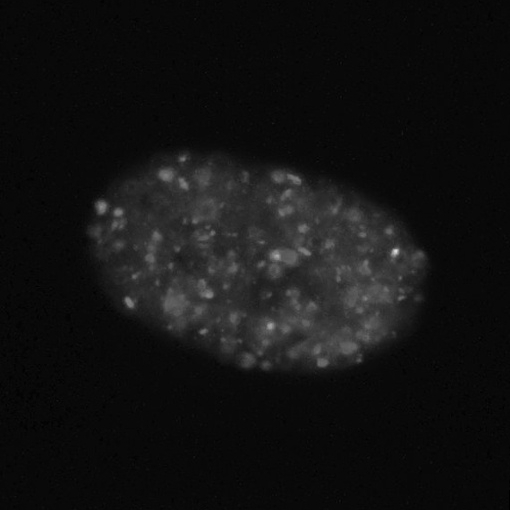
\includegraphics[width=\myWidth\columnwidth]{figures/cell_database_gray/5gray.jpg}
		\label{fig:5gray}
	}
	\subfigure[Image 6]
	{
		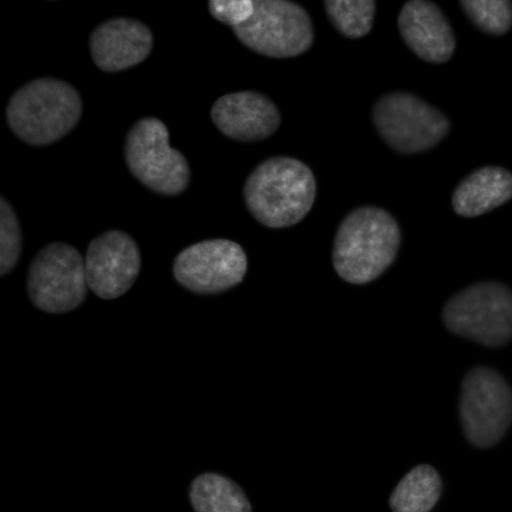
\includegraphics[width=\myWidth\columnwidth]{figures/cell_database_gray/6gray.jpg}
		\label{fig:6gray}
	}
	\caption{Images from tuning set.}
	\label{fig:tuningset}
\end{figure}

Since the curves energy functions, $E^i(0)$ and $E^i(1)$, can be tuned relative to a fixed value for $\mu$, which this would not impact significantly on the range of possible solution sets, we set $\mu=1$ in all our manual parameter tuning. We use a stopping criterion of $\epsilon=1\times10^{-3}$. We compared the effect of using Otsu binarization, K-means ($k=2$) and Expectation-Maximisation for Gaussian Mixture Modelling (EMGMM) with ($k=2$) for generating the initial means, $c0$ and $c_1$. The values used for $\alpha \in [1, 10, 20, 30, 40, 45, 50]$ and the values used for $\lambda_1 \in [50, 100, 150, 200, 400, 800]$. The remaining parameters were calculated from $\mu$, $\alpha$ and $\lambda_1$.

As final results we take the means of the final segmentation for the background and foreground regions. An acceptable solution was one that achieved at least $70\%$ of the final means from the ground truth for each region. From the acceptable results, we calculate the values for $p_e$, \Cref{eq:pe}, and $h$, \Cref{eq:h}.
The means for each image can vary greatly.
To put the values of $p_e$ and $h$ into a relative perspective, they are shown as a fraction of the distance between $c_0$ and $c_1$.
Let $k_p \in (0,1)$ be the fraction of the distance $p_e-c_0$ and $c_1-c_0$ as illustrated in \Cref{fig:kp}.
Let $k_h \in (k_h,1)$ be the fraction of the distance $h-c_0$ and $c_1-c_0$ as illustrated in \Cref{fig:kh}, we have $0 < k_p < k_h$.

\begin{figure}[!h]
	\centering
	\begin{tikzpicture}[scale=1]
	\draw[-] (0,0) -- (15,0) node[right] {$p$};
	\draw[shift={(3,0)}] (0pt,4pt) -- (0pt,-4pt) node[below] {$c_0$};
	\draw[shift={(12,0)}] (0pt,4pt) -- (0pt,-4pt) node[below] {$c_1$};
	
	\draw[dashed,black] (5.0,1.5) -- (5.0,-0.3) node[below] {$p_e$};
	
	\draw[black,*-*,thick] (5.0,0.5) -- (4.0,0.5) node[above] {$k_p(c_1-c_0)$} -- (3.0,0.5);
	
	\end{tikzpicture}
	\caption{$p_e$ as a fraction of the distance between $c_0$ and $c_1$.}
	\label{fig:kp}
\end{figure}

\begin{figure}[!h]
	\centering
	\begin{tikzpicture}[scale=1]
	\draw[-] (0,0) -- (15,0) node[right] {$p$};
	\draw[shift={(3,0)}] (0pt,4pt) -- (0pt,-4pt) node[below] {$c_0$};
	\draw[shift={(12,0)}] (0pt,4pt) -- (0pt,-4pt) node[below] {$c_1$};
	
	\draw[dashed,black] (9.0,1.5) -- (9.0,-0.3) node[below] {$h$};
	
	\draw[black,*-*,thick] (9.0,0.5) -- (6.0,0.5) node[above] {$k_h(c_1-c_0)$} -- (3.0,0.5);
	\draw[black,*-*,thick] (9.0,0.5) -- (10.5,0.5) node[above] {$(1-k_h)(c_1-c_0)$} -- (12.0,0.5);
	\end{tikzpicture}
	\caption{$h$ as a fraction of the distance between $c_0$ and $c_1$.}
	\label{fig:kh}
\end{figure}

Upon comparing the initial means and final means for the acceptable segmentation results, it was noted the the values of the initial means are larger. This is due to over-segmentation produced by Otsu, K-means and EMGMM clustering. A na{\"i}ve approach to shifting the initial means closer to the final means is to dilate the initial mask. This pushes the boundaries of the contour for the object to accept the lower intensity neighbouring pixels, as well as remove these relatively higher values from the background mask. If we are able to make a better guess to the initial means, then the fewer iterations are needed to converge within the stopping criterion.

To determine the optimal dilation size, we compare the difference of the mean values for each image, for the acceptable segmentation results only. We use an elliptical element for dilation and the size of the dilation ranged from $r \in [1, 2, 3, 5 , 7, 9]$. A dilation size of 3 for a elliptical dilation element results in mean values that are closest to the average final means.

When defining the values for $p_e$ and $h$ implicitly and $k_p$ and $k_h$ respectively, we find the updated equation for determining $\alpha$ is simplified to
\begin{equation}
	\alpha = \left( \frac{1-k_p}{k_p} \right)^2
	\label{eq:alphafromkp}
\end{equation}

%\begin{equation}\begin{split}
%	\alpha-1 = \frac{1-2k_p+k_p^2-k_p^2}{k_p^2} = \frac{1-2k_p}{k_p^2}
%\end{split}\end{equation}

%The point where the energies are equal can be calculated as:
%\begin{equation}
%	p_e = c_0 + k_p(c_1-c_0)
%\end{equation}

%Following from \Cref{eq:lambda1approximation}
%
%\begin{equation*}
%	h = (c_1-c_0)^2\left( \left( \frac{1-2k_p}{k_p^2} \right)k_h^2 +2k_h -1 \right)
%\end{equation*}

The weighting parameter $\lambda_1$ can be calculated as

%\begin{equation}
%	\lambda_1 = \frac{\mu \left( 2\sqrt{2}+4\right)}{(c_1-c_0)^2\left( \left( \frac{1-2k_p}{k_p^2} \right)k_h^2 +2k_h -1 \right)}
%	\label{eq:lambda1fromkpandkh}
%\end{equation}
\begin{equation}
\lambda_1 = \frac{C\mu}{(c_1-c_0)^2\left( \left( \frac{1-2k_p}{k_p^2} \right)k_h^2 +2k_h -1 \right)}
\label{eq:lambda1fromkpandkh}
\end{equation}

%The parameters $\alpha$ and $\lambda_1$, in the proposed parameter estimation method, depend greatly on predicting good final means, $c_0$ and $c_1$, as well as $p_e$ and $h$ for the ideal segmentation.

For determining $\alpha$ we found the average of all $k_p$ for all acceptable segmentations. This is calculated to be
\begin{equation*}
	k_p = 0.154494.
\end{equation*}
From this we can calculate the value for $\alpha$ immediately using \Cref{eq:alphafromkp}. This turns out to be
\begin{equation}
	\alpha = 29.9509.
\end{equation}
Similarly, to determine $h$ we find the average of all $k_h$ for all acceptable segmentations. This is calculated to be
\begin{equation*}
	k_h = 0.412737.
\end{equation*}
An appropriate value for $\lambda_1$ depends on $c_0$ and $c_1$, as can be seen in \Cref{eq:lambda1fromkpandkh}, which can only be determined after the inital means are generated.

\subsection{Parameter Estimation Process}
We now present the final parameter estimation process. The parameters whose values are fixed are
\begin{enumerate}
	\item $\mu=1$
	\item $k_p = 0.154494$
	\item $k_h = 0.412737$
	\item $\alpha = 29.9509$
\end{enumerate}
We first segment the image to determine the initial $c_0$ and $c_1$. We can then calculate $\lambda_1$ using \Cref{eq:lambda1fromkpandkh}. Finally, we can calculate $\lambda_0$ using \Cref{eq:l0l1dependancy}.
The remaining parameter is the stopping criterion $\epsilon$ which we set to  $1 \times 10^{-3}$.

\section{Experimental Results}
\label{sec:Expresults}
We compare our results to two previously published parameter settings.
%The first is the parameter settings used El Zehiry \textit{et al.} \citep{ElZehiry2007}, which is where the Chan-Vese Graph Cut technique was first published.
Their results showed excellent segmentation output on synthetic images and mammography images with very high robustness against noise. They do not specify the noise type.
%The second parameter setting which we compete against is presented by Masaka \textit{et al.} \citep{Maska2013}.
Their parameter setting was based on a time-lapse series of fluorescence images. Their scheme is a hybrid of algorithms designed to segment whole fluorescent cells; however, we use the parameter setting they have presented for segmentation only. Their parameter setting was obtained by minimising the Jaccard coefficient over the time-lapse series.
%Their results show a greater area of cell detection and smoother boundaries; although, the smoother contours are a result of CED-ORI \citep{Weickert2002} which is part of the scheme before segmentation.

To generate the initial means we used the EMGMM with $k=2$ which was followed by an elliptical dilation of size $3$.
The results of all segmentation scheme are shown from \Cref{fig:testresult188} to \Cref{fig:testresult42451}.

In \Cref{tab:segmentationefficiency}, which compares the segmentation efficiency of each method, we differentiate between methods on the same image as follows:

\textbf{[imageno]-[method]}, 

where \textit{imageno} goes from $1$ to $25$ and \textit{method} is defined as follows:
\begin{enumerate}
	\item [\textbf{n}] - using parameter setting presented by El-Zehiry \textit{et. al} %\citep{ElZehiry2007}.
	\item [\textbf{m}] - using parameter setting presented by Masaka \textit{et. al} %\citep{Maska2013}.
	\item [\textbf{d}] - Proposed method with parameters estimated from an initial EMGMM segmentation with $k=2$ and an elliptical dilation of $3px$.
\end{enumerate}

In \Cref{tab:segmentationefficiency} we compare the accuracy and MCC of each segmented result for each scheme. Accuracy is the fraction of the pixels that are correctly classified from among all pixels. MCC is the \textit{Matthews Correlation Coefficient} and is a more accurate measure of accuracy when comparing classes whose sizes differ greatly. 

We used a 8-connected graph for all methods.

\begin{longtabu}[!h] {|c|c|c|c|c|c|c|}
	\caption{Segmentation Efficiency.} \label{tab:segmentationefficiency} \\
	\hline \multirow{2}{*}{Image} & \multicolumn{2}{c|}{El-Zehiry \textit{et. al}} &  \multicolumn{2}{c|}{Masaka \textit{et. al}} &  \multicolumn{2}{c|}{Proposed} \\
	\hhline{~------}
	& Accuracy & MCC & Accuracy & MCC &Accuracy & MCC  \\
	\hline	1 & 0.770111 & 0.626140 & 0.967117 & 0.934010  & 0.959427 & 0.919468 \\
	\hline	2 & 0.747253 & 0.416180 & 0.335449 & -0.008374 & 0.862671 & 0.748686 \\
	\hline	5 & 0.912262 & 0.811918 & 0.851883 & 0.739708 & 0.916992 & 0.842769	\\
	\hline	6 & 0.515686 & 0.300907 & 0.603195 & 0.028915 & 0.966156 & 0.931253	\\
	\hline	9 & 0.886490 & 0.589732 & 0.938583 & 0.834732 & 0.990768 & 0.970635	\\ 
	\hline	12& 0.806732 & 0.519903 & 0.309845 & 0.060018 & 0.905685 & 0.808358	\\ 
	\hline	15& 0.962357 & 0.507270 & 0.098129 & 0.051537 & 0.990158 & 0.911074	\\
	\hline	17& 0.888229 & 0.452365	& 0.150055 & 0.020336 & 0.915009 & 0.733933	\\
	\hline	18& 0.595612 & 0.384991 & 0.567032 & NaN      & 0.960739 & 0.922580	\\
	\hline	19& 0.852585 & 0.559970 & 0.570099 & 0.393942 & 0.975266 & 0.933388	\\
	\hline	20& 0.914856 & 0.719637 & 0.679703 & 0.479944 & 0.966690 & 0.904878	\\
	\hline	21& 0.913818 & 0.678954 & 0.181793 & 0.035231 & 0.967438 & 0.885155	\\
	\hline	22& 0.703156 & 0.469557 & 0.449310 & NaN      & 0.981735 & 0.963345	\\
	\hline	24& 0.921356 & 0.562635 & 0.136047 & 0.047223 & 0.882690 & 0.661018	\\
	\hline	25& 0.573715 & 0.296608 & 0.511276 & NaN      & 0.959915 & 0.920148	\\
	\hline 
\end{longtabu} 

\begin{longtable}{|c|c|c|}
	\caption{Overall Segmentation Efficiency.} \label{tab:overallsegmentationefficiency}\\
	\hline 
	\multirow{2}{*}{Method} & \multicolumn{2}{c|}{Accuracy}  \\ 
	\hhline{~--}
	& Mean & Std. Dev   \\ 
	\hline	El-Zehiry \textit{et al.} %\citep{ElZehiry2007}	
	& 0.805732	&	0.151199	\\
	\hline Maska \textit{et al.} %\citep{Maska2013}	
	&	0.547369	&	0.321099\\
	\hline	Proposed &	0.935329	&	0.064493	\\
	\hline
\end{longtable} 

The general parameter settings by El-Zehiry \textit{et al.} % \citep{ElZehiry2007}  
clearly outperform by the parameter settings presented by Masaka \textit{et al.} %\citep{Maska2013} 
by a 25.8363\% difference in accuracy. However, the proposed method boasts an increase of 12.9597\% above El-Zehiry's parameter settings. The proposed method is also much more stable over a greater variety of fluorescence images, as can be seen by the standard deviation of accuracy shown in \Cref{tab:overallsegmentationefficiency}.












% needed in second column of first page if using \IEEEpubid
%\IEEEpubidadjcol

% An example of a floating figure using the graphicx package.
% Note that \label must occur AFTER (or within) \caption.
% For figures, \caption should occur after the \includegraphics.
% Note that IEEEtran v1.7 and later has special internal code that
% is designed to preserve the operation of \label within \caption
% even when the captionsoff option is in effect. However, because
% of issues like this, it may be the safest practice to put all your
% \label just after \caption rather than within \caption{}.
%
% Reminder: the "draftcls" or "draftclsnofoot", not "draft", class
% option should be used if it is desired that the figures are to be
% displayed while in draft mode.
%
%\begin{figure}[!t]
%\centering
%\includegraphics[width=2.5in]{myfigure}
% where an .eps filename suffix will be assumed under latex, 
% and a .pdf suffix will be assumed for pdflatex; or what has been declared
% via \DeclareGraphicsExtensions.
%\caption{Simulation Results}
%\label{fig_sim}
%\end{figure}

% Note that IEEE typically puts floats only at the top, even when this
% results in a large percentage of a column being occupied by floats.


% An example of a double column floating figure using two subfigures.
% (The subfig.sty package must be loaded for this to work.)
% The subfigure \label commands are set within each subfloat command, the
% \label for the overall figure must come after \caption.
% \hfil must be used as a separator to get equal spacing.
% The subfigure.sty package works much the same way, except \subfigure is
% used instead of \subfloat.
%
%\begin{figure*}[!t]
%\centerline{\subfloat[Case I]\includegraphics[width=2.5in]{subfigcase1}%
%\label{fig_first_case}}
%\hfil
%\subfloat[Case II]{\includegraphics[width=2.5in]{subfigcase2}%
%\label{fig_second_case}}}
%\caption{Simulation results}
%\label{fig_sim}
%\end{figure*}
%
% Note that often IEEE papers with subfigures do not employ subfigure
% captions (using the optional argument to \subfloat), but instead will
% reference/describe all of them (a), (b), etc., within the main caption.


% An example of a floating table. Note that, for IEEE style tables, the 
% \caption command should come BEFORE the table. Table text will default to
% \footnotesize as IEEE normally uses this smaller font for tables.
% The \label must come after \caption as always.
%
%\begin{table}[!t]
%% increase table row spacing, adjust to taste
%\renewcommand{\arraystretch}{1.3}
% if using array.sty, it might be a good idea to tweak the value of
% \extrarowheight as needed to properly center the text within the cells
%\caption{An Example of a Table}
%\label{table_example}
%\centering
%% Some packages, such as MDW tools, offer better commands for making tables
%% than the plain LaTeX2e tabular which is used here.
%\begin{tabular}{|c||c|}
%\hline
%One & Two\\
%\hline
%Three & Four\\
%\hline
%\end{tabular}
%\end{table}


% Note that IEEE does not put floats in the very first column - or typically
% anywhere on the first page for that matter. Also, in-text middle ("here")
% positioning is not used. Most IEEE journals use top floats exclusively.
% Note that, LaTeX2e, unlike IEEE journals, places footnotes above bottom
% floats. This can be corrected via the \fnbelowfloat command of the
% stfloats package.


\section{Conclusion}
\label{sec:Conc}
Fluorescence images are hugely diverse; even so of the images within the fields of cellular biology and medicine. The design of a general and  automatic segmentation method is not a trivial exercise; and, it is much needed.

We have presented a novel parameter estimation technique which is able to tune the parameters of the graph-cut application of the Chan-Vese segmentation method, to the specific image.
This is a huge contrast in comparison to the fixed parameter settings proposed by El-Zehiry \textit{et al.} %\citep{ElZehiry2007} 
and Masaka \textit{et al.} %\citep{Maska2013}.
Our method, does however, rely on the strong assumption that the initial means obtained from the initial unsupervised segmentation scheme is relatively close to the final means. 
Fortunately though, in the domain of biological and medical fluorescence images, the unsupervised segmentation results obtained from an Otsu, K-means or EMGMM clustering is close enough to outperform the competitor parameter settings. We have shown that an EMGMM clustering and a dilation of 3 pixels, with an elliptical dilation element, provides the best approximation to the final means which results in an average of 93.5329\% classification accuracy. Given the diversity of fluorescence images in the test set, this is a very pleasing result, especially when compared to the competitor parameter settings by El-Zehiry \textit{et al.} %\citep{ElZehiry2007} 
which showed an average of 80.5732\% and Masaka \textit{et al.} %\citep{Maska2013} 
which showed an average of 54.7369\%.
%Furthermore, considering the fact that it is not possible, for even the same professional, to consistently manually segment an image the same everytime, and that greater variation in groundtruths will result from many professionals, we can see that even a 10\% variation in groundtruths will result in the proposed scheme superseding the other schemes. This further shows the robustness of the algorithm.

Once the initial means have been obtained, the parameters are adapted to the image by direct calculation by means of the \textit{relationship variables and formulae}. These relationship variables and formulae encode the important relation of the parameters with each other. This allows the  ability to adapt the parameter settings according to the properties of the image. These resutling parameters only allow high segmentation accuracy if the image has the properties that are encoded in the relationship variables and formulae.

The relationship formulae only take into account the infomation from the intensity of the image. Other infomation, such as texture, can be incorporated into the formulae as well. This will include adapting the graph to hold this infomation so that it can be accounted for in the energy function.

\def \myWidth {0.2}
%%%%%%%%%%%%%%%%%%%%%%%%%%%%%%%%%%%%%%%%%%%%%%%%%%%%%%%
% 188
\begin{figure}[!h]
	\centering
	\subfigure[Original.]
	{
		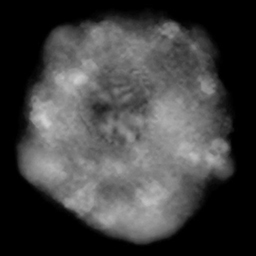
\includegraphics[width=\myWidth\columnwidth]{figures/cell_database_gray/188gray}
		\label{fig:orig188}
	}
	\subfigure[El-Zehiry \textit{et al}.]
	{
		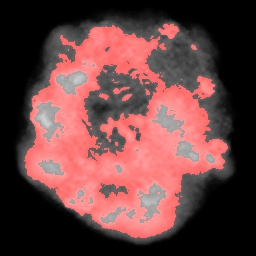
\includegraphics[width=\myWidth\columnwidth]{figures/propsedcv/def/def188}
		\label{fig:default188}
	}
	\subfigure[Masaka \textit{et al}.]
	{
		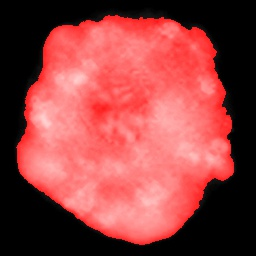
\includegraphics[width=\myWidth\columnwidth]{figures/propsedcv/shapetrack/shapetrack188}
		\label{fig:shapetrack188}
	}
	\subfigure[Proposed. %$\mu=1$, $\alpha=29.9509$, 
	$\lambda_1=8.17148$.]
	{
		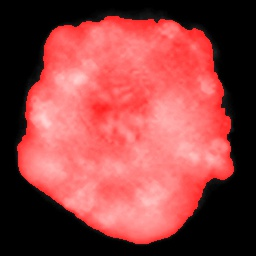
\includegraphics[width=\myWidth\columnwidth]{figures/propsedcv/dilated/emgmm2188finmask}
		\label{fig:propsedCVemgmmdilate188}
	}
	\caption{Image 1 from test set segmentation results.}
	\label{fig:testresult188}
\end{figure}
%%%%%%%%%%%%%%%%%%%%%%%%%%%%%%%%%%%%%%%%%%%%%%%%%%%%%%%
% 195
\begin{figure}[!h]
	\centering
	\subfigure[Original.]
	{
		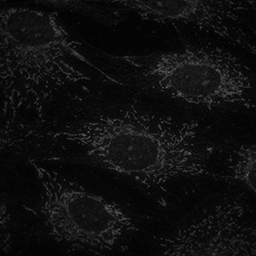
\includegraphics[width=\myWidth\columnwidth]{figures/cell_database_gray/195gray}
		\label{fig:orig195}
	}
	\subfigure[El-Zehiry \textit{et al}.]
	{
		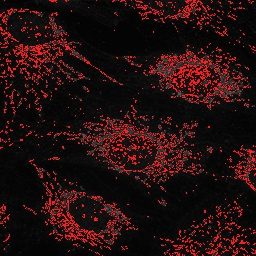
\includegraphics[width=\myWidth\columnwidth]{figures/propsedcv/def/def195}
		\label{fig:default195}
	}
	\subfigure[Masaka \textit{et al}.]
	{
		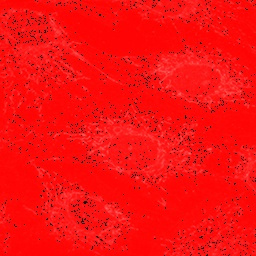
\includegraphics[width=\myWidth\columnwidth]{figures/propsedcv/shapetrack/shapetrack195}
		\label{fig:shapetrack195}
	}
	\subfigure[Proposed. %$\mu=1$, $\alpha=29.9509$, 
	$\lambda_1=606.199$.]
	{
		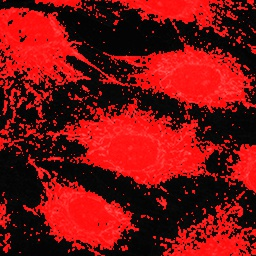
\includegraphics[width=\myWidth\columnwidth]{figures/propsedcv/dilated/emgmm2195finmask}
		\label{fig:propsedCVemgmmdilate195}
	}
	\caption{Image 2 from test set segmentation results.}
	\label{fig:testresult195}
\end{figure}
%%%%%%%%%%%%%%%%%%%%%%%%%%%%%%%%%%%%%%%%%%%%%%%%%%%%%%%
% 1265
\begin{figure}[!h]
	\centering
	\subfigure[Original.]
	{
		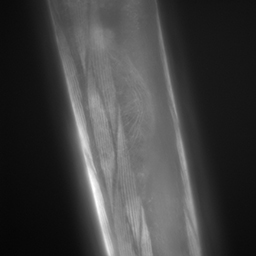
\includegraphics[width=\myWidth\columnwidth]{figures/cell_database_gray/1265gray}
		\label{fig:orig1265}
	}
	\subfigure[El-Zehiry \textit{et al}.]
	{
		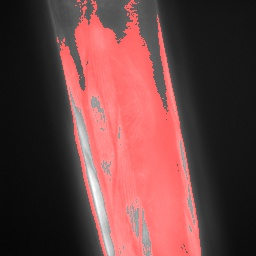
\includegraphics[width=\myWidth\columnwidth]{figures/propsedcv/def/def1265}
		\label{fig:default1265}
	}
	\subfigure[Masaka \textit{et al}.]
	{
		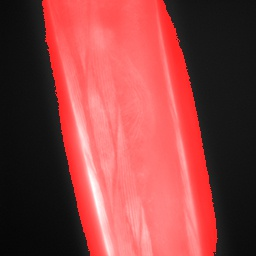
\includegraphics[width=\myWidth\columnwidth]{figures/propsedcv/shapetrack/shapetrack1265}
		\label{fig:shapetrack1265}
	}
	\subfigure[Proposed. $\lambda_1=11.2011$.]
	{
		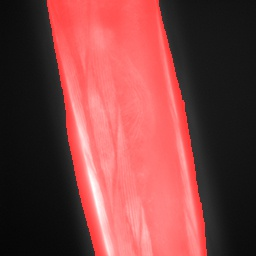
\includegraphics[width=\myWidth\columnwidth]{figures/propsedcv/dilated/emgmm21265finmask}
		\label{fig:propsedCVemgmmdilate1265}
	}
	\caption{Image 5 from test set segmentation results.}
	\label{fig:testresult1265}
\end{figure}
%%%%%%%%%%%%%%%%%%%%%%%%%%%%%%%%%%%%%%%%%%%%%%%%%%%%%%%
% 10093
\begin{figure}[!h]
	\centering
	\subfigure[Original.]
	{
		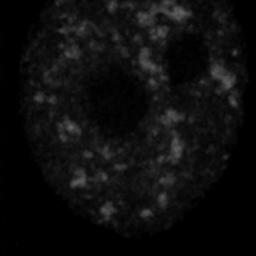
\includegraphics[width=\myWidth\columnwidth]{figures/cell_database_gray/10093gray}
		\label{fig:orig10093}
	}
	\subfigure[El-Zehiry \textit{et al}.]
	{
		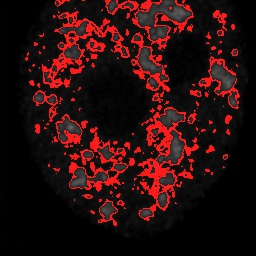
\includegraphics[width=\myWidth\columnwidth]{figures/propsedcv/def/def10093}
		\label{fig:default10093}
	}
	\subfigure[Masaka \textit{et al}.]
	{
		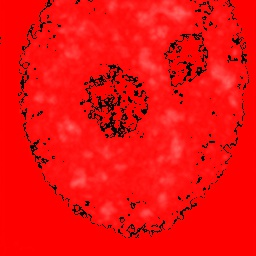
\includegraphics[width=\myWidth\columnwidth]{figures/propsedcv/shapetrack/shapetrack10093}
		\label{fig:shapetrack10093}
	}
	\subfigure[Proposed. $\lambda_1=161.108$.]
	{
		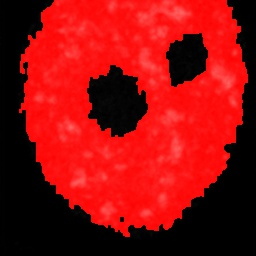
\includegraphics[width=\myWidth\columnwidth]{figures/propsedcv/dilated/emgmm210093finmask}
		\label{fig:propsedCVemgmmdilate10093}
	}
	\caption{Image 6 from test set segmentation results.}
	\label{fig:testresult10093}
\end{figure}
%%%%%%%%%%%%%%%%%%%%%%%%%%%%%%%%%%%%%%%%%%%%%%%%%%%%%%%
% 12294
\begin{figure}[!h]
	\centering
	\subfigure[Original.]
	{
		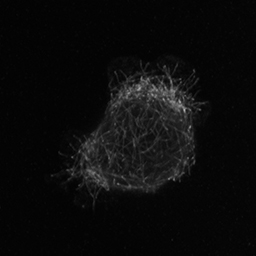
\includegraphics[width=\myWidth\columnwidth]{figures/cell_database_gray/12294gray}
		\label{fig:orig12294}
	}
	\subfigure[El-Zehiry \textit{et al}.]
	{
		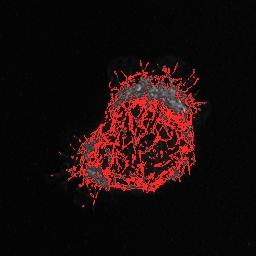
\includegraphics[width=\myWidth\columnwidth]{figures/propsedcv/def/def12294}
		\label{fig:default12294}
	}
	\subfigure[Masaka \textit{et al}.]
	{
		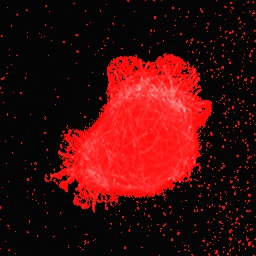
\includegraphics[width=\myWidth\columnwidth]{figures/propsedcv/shapetrack/shapetrack12294}
		\label{fig:shapetrack12294}
	}
	\subfigure[Proposed. $\lambda_1=146.629$.]
	{
		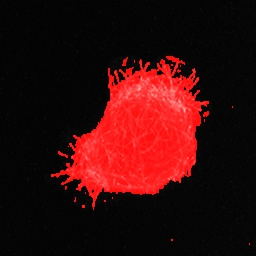
\includegraphics[width=\myWidth\columnwidth]{figures/propsedcv/dilated/emgmm212294finmask}
		\label{fig:propsedCVemgmmdilate12294}
	}
	\caption{Image 9 from test set segmentation results.}
	\label{fig:testresult12294}
\end{figure}
%%%%%%%%%%%%%%%%%%%%%%%%%%%%%%%%%%%%%%%%%%%%%%%%%%%%%%%
% 13438
\begin{figure}[!h]
	\centering
	\subfigure[Original.]
	{
		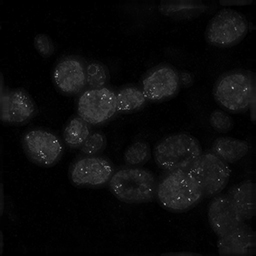
\includegraphics[width=\myWidth\columnwidth]{figures/cell_database_gray/13438gray}
		\label{fig:orig13438}
	}
	\subfigure[El-Zehiry \textit{et al}.]
	{
		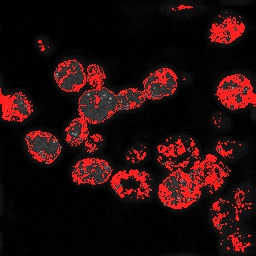
\includegraphics[width=\myWidth\columnwidth]{figures/propsedcv/def/def13438}
		\label{fig:default13438}
	}
	\subfigure[Masaka \textit{et al}.]
	{
		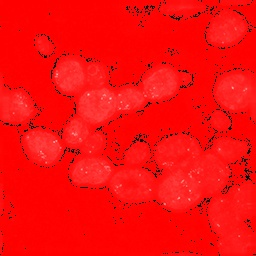
\includegraphics[width=\myWidth\columnwidth]{figures/propsedcv/shapetrack/shapetrack13438}
		\label{fig:shapetrack13438}
	}
	\subfigure[Proposed. $\lambda_1=160.407$.]
	{
		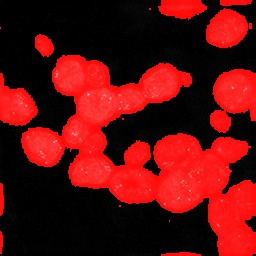
\includegraphics[width=\myWidth\columnwidth]{figures/propsedcv/dilated/emgmm213438finmask}
		\label{fig:propsedCVemgmmdilate13438}
	}
	\caption{Image 12 from test set segmentation results.}
	\label{fig:testresult13438}
\end{figure}
%%%%%%%%%%%%%%%%%%%%%%%%%%%%%%%%%%%%%%%%%%%%%%%%%%%%%%%
% 21749
\begin{figure}[!h]
	\centering
	\subfigure[Original.]
	{
		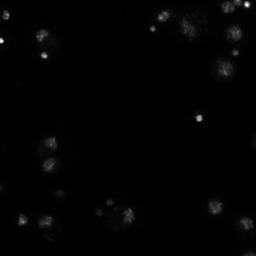
\includegraphics[width=\myWidth\columnwidth]{figures/cell_database_gray/21749gray}
		\label{fig:orig21749}
	}
	\subfigure[El-Zehiry \textit{et al}.]
	{
		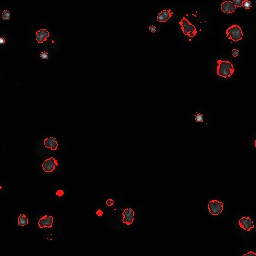
\includegraphics[width=\myWidth\columnwidth]{figures/propsedcv/def/def21749}
		\label{fig:default21749}
	}
	\subfigure[Masaka \textit{et al}.]
	{
		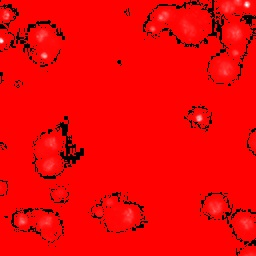
\includegraphics[width=\myWidth\columnwidth]{figures/propsedcv/shapetrack/shapetrack21749}
		\label{fig:shapetrack21749}
	}
	\subfigure[Proposed. $\lambda_1=860.426$.]
	{
		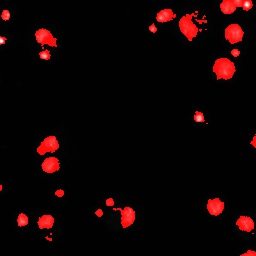
\includegraphics[width=\myWidth\columnwidth]{figures/propsedcv/dilated/emgmm221749finmask}
		\label{fig:propsedCVemgmmdilate21749}
	}
	\caption{Image 15 from test set segmentation results.}
	\label{fig:testresult21749}
\end{figure}
%%%%%%%%%%%%%%%%%%%%%%%%%%%%%%%%%%%%%%%%%%%%%%%%%%%%%%%
% 32140
\begin{figure}[!h]
	\centering
	\subfigure[Original.]
	{
		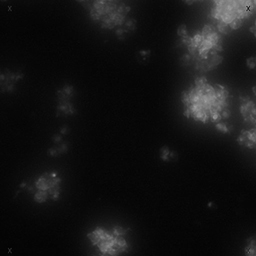
\includegraphics[width=\myWidth\columnwidth]{figures/cell_database_gray/32140gray}
		\label{fig:orig32140}
	}
	\subfigure[El-Zehiry \textit{et al}.]
	{
		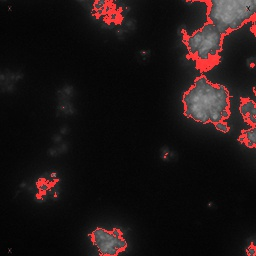
\includegraphics[width=\myWidth\columnwidth]{figures/propsedcv/def/def32140}
		\label{fig:default32140}
	}
	\subfigure[Masaka \textit{et al}.]
	{
		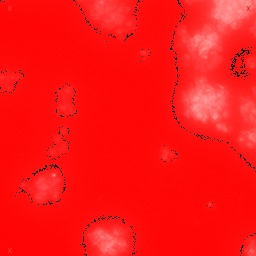
\includegraphics[width=\myWidth\columnwidth]{figures/propsedcv/shapetrack/shapetrack32140}
		\label{fig:shapetrack32140}
	}
	\subfigure[Proposed. $\lambda_1=43.33$.]
	{
		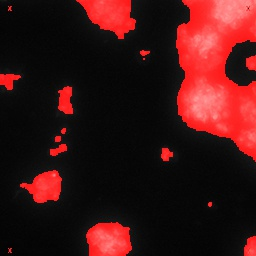
\includegraphics[width=\myWidth\columnwidth]{figures/propsedcv/dilated/emgmm232140finmask}
		\label{fig:propsedCVemgmmdilate32140}
	}
	\caption{Image 17 from test set segmentation results.}
	\label{fig:testresult32140}
\end{figure}
%%%%%%%%%%%%%%%%%%%%%%%%%%%%%%%%%%%%%%%%%%%%%%%%%%%%%%%
% 35278
\begin{figure}[!h]
	\centering
	\subfigure[Original.]
	{
		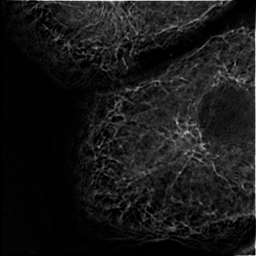
\includegraphics[width=\myWidth\columnwidth]{figures/cell_database_gray/35278gray}
		\label{fig:orig35278}
	}
	\subfigure[El-Zehiry \textit{et al}.]
	{
		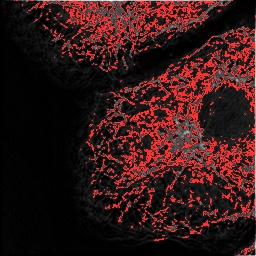
\includegraphics[width=\myWidth\columnwidth]{figures/propsedcv/def/def35278}
		\label{fig:default35278}
	}
	\subfigure[Masaka \textit{et al}.]
	{
		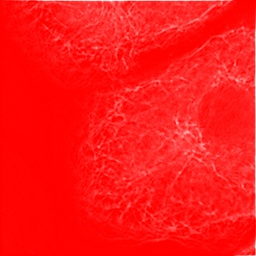
\includegraphics[width=\myWidth\columnwidth]{figures/propsedcv/shapetrack/shapetrack35278}
		\label{fig:shapetrack35278}
	}
	\subfigure[Proposed. $\lambda_1=85.0788$.]
	{
		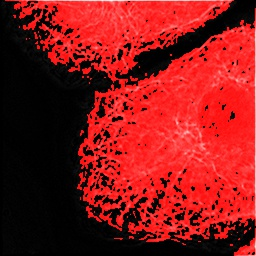
\includegraphics[width=\myWidth\columnwidth]{figures/propsedcv/dilated/emgmm235278finmask}
		\label{fig:propsedCVemgmmdilate35278}
	}
	\caption{Image 18 from test set segmentation results.}
	\label{fig:testresult35278}
\end{figure}
%%%%%%%%%%%%%%%%%%%%%%%%%%%%%%%%%%%%%%%%%%%%%%%%%%%%%%%
% 37338
\begin{figure}[!h]
	\centering
	\subfigure[Original.]
	{
		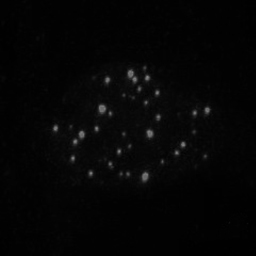
\includegraphics[width=\myWidth\columnwidth]{figures/cell_database_gray/37338gray}
		\label{fig:orig37338}
	}
	\subfigure[El-Zehiry \textit{et al}.]
	{
		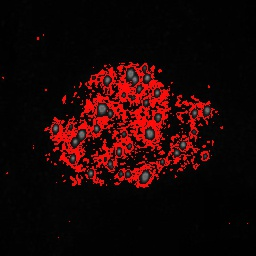
\includegraphics[width=\myWidth\columnwidth]{figures/propsedcv/def/def37338}
		\label{fig:default37338}
	}
	\subfigure[Masaka \textit{et al}.]
	{
		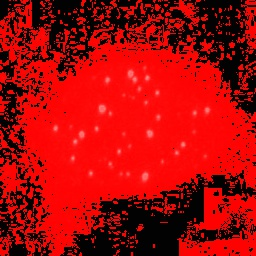
\includegraphics[width=\myWidth\columnwidth]{figures/propsedcv/shapetrack/shapetrack37338}
		\label{fig:shapetrack37338}
	}
	\subfigure[Proposed. $\lambda_1=309.766$.]
	{
		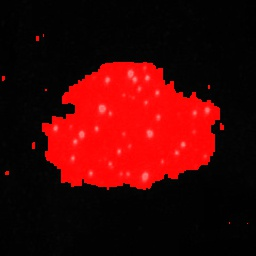
\includegraphics[width=\myWidth\columnwidth]{figures/propsedcv/dilated/emgmm237338finmask}
		\label{fig:propsedCVemgmmdilate37338}
	}
	\caption{Image 19 from test set segmentation results.}
	\label{fig:testresult37338}
\end{figure}
%%%%%%%%%%%%%%%%%%%%%%%%%%%%%%%%%%%%%%%%%%%%%%%%%%%%%%%
% 37339
\begin{figure}[!h]
	\centering
	\subfigure[Original.]
	{
		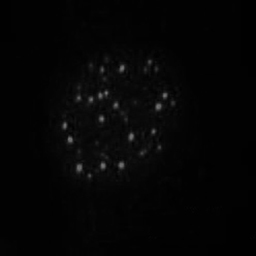
\includegraphics[width=\myWidth\columnwidth]{figures/cell_database_gray/37339gray}
		\label{fig:orig37339}
	}
	\subfigure[El-Zehiry \textit{et al}.]
	{
		\includegraphics[width=\myWidth\columnwidth]{figures/propsedcv/def/def37339}
		\label{fig:default37339}
	}
	\subfigure[Masaka \textit{et al}.]
	{
		\includegraphics[width=\myWidth\columnwidth]{figures/propsedcv/shapetrack/shapetrack37339}
		\label{fig:shapetrack37339}
	}
	\subfigure[Proposed. $\lambda_1=359.465$.]
	{
		\includegraphics[width=\myWidth\columnwidth]{figures/propsedcv/dilated/emgmm237339finmask}
		\label{fig:propsedCVemgmmdilate37339}
	}
	\caption{Image 20 from test set segmentation results.}
	\label{fig:testresult37339}
\end{figure}
%%%%%%%%%%%%%%%%%%%%%%%%%%%%%%%%%%%%%%%%%%%%%%%%%%%%%%%
% 38974
\begin{figure}[!h]
	\centering
	\subfigure[Original.]
	{
		\includegraphics[width=\myWidth\columnwidth]{figures/cell_database_gray/38974gray}
		\label{fig:orig38974}
	}
	\subfigure[El-Zehiry \textit{et al}.]
	{
		\includegraphics[width=\myWidth\columnwidth]{figures/propsedcv/def/def38974}
		\label{fig:default38974}
	}
	\subfigure[Masaka \textit{et al}.]
	{
		\includegraphics[width=\myWidth\columnwidth]{figures/propsedcv/shapetrack/shapetrack38974}
		\label{fig:shapetrack38974}
	}
	\subfigure[Proposed. $\lambda_1=359.465$.]
	{
		\includegraphics[width=\myWidth\columnwidth]{figures/propsedcv/dilated/emgmm238974finmask}
		\label{fig:propsedCVemgmmdilate38974}
	}
	\caption{Image 21 from test set segmentation results.}
	\label{fig:testresult38974}
\end{figure}
%%%%%%%%%%%%%%%%%%%%%%%%%%%%%%%%%%%%%%%%%%%%%%%%%%%%%%%
% 40217
\begin{figure}[!h]
	\centering
	\subfigure[Original.]
	{
		\includegraphics[width=\myWidth\columnwidth]{figures/cell_database_gray/40217gray}
		\label{fig:orig40217}
	}
	\subfigure[El-Zehiry \textit{et al}.]
	{
		\includegraphics[width=\myWidth\columnwidth]{figures/propsedcv/def/def40217}
		\label{fig:default40217}
	}
	\subfigure[Masaka \textit{et al}.]
	{
		\includegraphics[width=\myWidth\columnwidth]{figures/propsedcv/shapetrack/shapetrack40217}
		\label{fig:shapetrack40217}
	}
	\subfigure[Proposed. $\lambda_1=38.837$.]
	{
		\includegraphics[width=\myWidth\columnwidth]{figures/propsedcv/dilated/emgmm240217finmask}
		\label{fig:propsedCVemgmmdilate40217}
	}
	\caption{Image 22 from test set segmentation results.}
	\label{fig:testresult40217}
\end{figure}
%%%%%%%%%%%%%%%%%%%%%%%%%%%%%%%%%%%%%%%%%%%%%%%%%%%%%%%
% 41066
\begin{figure}[!h]
	\centering
	\subfigure[Original.]
	{
		\includegraphics[width=\myWidth\columnwidth]{figures/cell_database_gray/41066gray}
		\label{fig:orig41066}
	}
	\subfigure[El-Zehiry \textit{et al}.]
	{
		\includegraphics[width=\myWidth\columnwidth]{figures/propsedcv/def/def41066}
		\label{fig:default41066}
	}
	\subfigure[Masaka \textit{et al}.]
	{
		\includegraphics[width=\myWidth\columnwidth]{figures/propsedcv/shapetrack/shapetrack41066}
		\label{fig:shapetrack41066}
	}
	\subfigure[Proposed. $\lambda_1=249.515$.]
	{
		\includegraphics[width=\myWidth\columnwidth]{figures/propsedcv/dilated/emgmm241066finmask}
		\label{fig:propsedCVemgmmdilate41066}
	}
	\caption{Image 24 from test set segmentation results.}
	\label{fig:testresult41066}
\end{figure}
%%%%%%%%%%%%%%%%%%%%%%%%%%%%%%%%%%%%%%%%%%%%%%%%%%%%%%%
% 42451
\begin{figure}[!h]
	\centering
	\subfigure[Original.]
	{
		\includegraphics[width=\myWidth\columnwidth]{figures/cell_database_gray/42451gray}
		\label{fig:orig42451}
	}
	\subfigure[El-Zehiry \textit{et al}.]
	{
		\includegraphics[width=\myWidth\columnwidth]{figures/propsedcv/def/def42451}
		\label{fig:default42451}
	}
	\subfigure[Masaka \textit{et al}.]
	{
		\includegraphics[width=\myWidth\columnwidth]{figures/propsedcv/shapetrack/shapetrack42451}
		\label{fig:shapetrack42451}
	}
	\subfigure[Proposed. $\lambda_1=118.726$.]
	{
		\includegraphics[width=\myWidth\columnwidth]{figures/propsedcv/dilated/emgmm242451finmask}
		\label{fig:propsedCVemgmmdilate42451}
	}
	\caption{Image 25 from test set segmentation results.}
	\label{fig:testresult42451}
\end{figure}




% if have a single appendix:
%\appendix[Proof of the Zonklar Equations]
% or
%\appendix  % for no appendix heading
% do not use \section anymore after \appendix, only \section*
% is possibly needed

% use appendices with more than one appendix
% then use \section to start each appendix
% you must declare a \section before using any
% \subsection or using \label (\appendices by itself
% starts a section numbered zero.)
%


%\appendices
%\section{Proof of the First Zonklar Equation}
%Some text for the appendix.

% use section* for acknowledgement
%\section*{Acknowledgment}
%
%
%The authors would like to thank...


% Can use something like this to put references on a page
% by themselves when using endfloat and the captionsoff option.
\ifCLASSOPTIONcaptionsoff
  \newpage
\fi

\pagebreak{4}

% trigger a \newpage just before the given reference
% number - used to balance the columns on the last page
% adjust value as needed - may need to be readjusted if
% the document is modified later
%\IEEEtriggeratref{8}
% The "triggered" command can be changed if desired:
%\IEEEtriggercmd{\enlargethispage{-5in}}

% references section

% can use a bibliography generated by BibTeX as a .bbl file
% BibTeX documentation can be easily obtained at:
% http://www.ctan.org/tex-archive/biblio/bibtex/contrib/doc/
% The IEEEtran BibTeX style support page is at:
% http://www.michaelshell.org/tex/ieeetran/bibtex/
%\bibliographystyle{IEEEtran}
% argument is your BibTeX string definitions and bibliography database(s)
%\bibliography{IEEEabrv,../bib/paper}
%
% <OR> manually copy in the resultant .bbl file
% set second argument of \begin to the number of references
% (used to reserve space for the reference number labels box)
\begin{thebibliography}{1}

\bibitem{IEEEhowto:kopka}
H.~Kopka and P.~W. Daly, \emph{A Guide to \LaTeX}, 3rd~ed.\hskip 1em plus
  0.5em minus 0.4em\relax Harlow, England: Addison-Wesley, 1999.

\end{thebibliography}

% biography section
% 
% If you have an EPS/PDF photo (graphicx package needed) extra braces are
% needed around the contents of the optional argument to biography to prevent
% the LaTeX parser from getting confused when it sees the complicated
% \includegraphics command within an optional argument. (You could create
% your own custom macro containing the \includegraphics command to make things
% simpler here.)
%\begin{biography}[{\includegraphics[width=1in,height=1.25in,clip,keepaspectratio]{mshell}}]{Michael Shell}
% or if you just want to reserve a space for a photo:

%\begin{IEEEbiography}[{\includegraphics[width=1in,height=1.25in,clip,keepaspectratio]{picture}}]{John Doe}
%\blindtext
%\end{IEEEbiography}

% You can push biographies down or up by placing
% a \vfill before or after them. The appropriate
% use of \vfill depends on what kind of text is
% on the last page and whether or not the columns
% are being equalized.

%\vfill

% Can be used to pull up biographies so that the bottom of the last one
% is flush with the other column.
%\enlargethispage{-5in}



% that's all folks
\end{document}


